\documentclass{article}
\usepackage[utf8]{inputenc}
\title{Lecture 10 low rank models}
\author{wbg231 }
\date{December 2022}
\newcommand{\R}{$\mathbb{R}$}
\newcommand{\B}{$\beta$}
\newcommand{\A}{$\alpha$}
\newcommand{\D}{\Delta}

\newcommand{\avector}[2]{(#1_2,\ldots,#1_{#2})}
\newcommand{\makedef}[2]{$\textbf{#1}$:#2 }
\usepackage{tikz,graphicx,hyperref,amsmath,amsfonts,amscd,amssymb,bm,cite,epsfig,epsf,url}

\begin{document}

\maketitle

\section*{introduction}
\begin{itemize}
\item the prof stopped making videos so form now on these are going to be text book notes 
\item \href{https://brightspace.nyu.edu/content/enforced/249915-794-1234_SP23DS-GAMATH-GA28403001005/notes/pca.pdf}{link}
\item up to now we have seen datasets where each data point is associated with a single entity 
\item now we are going to talk about cases where the data set are associated with two different entities
\item we represent such data as entries in a matrix $D$ for each enters $D[i,j]$ column i row j indicate the entries associated to each data point 
\item for example in recommender systems $D[i,j]$ would correspond to the rating user i gave to product j. 
\item for example in genomics $D[i,j]$ would correspond to the expression of gene i in cell j 
\item also i may use $D[i,j]$ and $D_{i.j}$ interchangeably 
\item in order to analyze such data it is often useful to represent each data point in terms of a small number of factors. 
\item this can be done by fitting the data using a low rank approximation 
\subsection*{movie example}
\item consider a matrix of movie rating $D\in \mathbb{R}^{n_1\times n_2}$ where $D_{i,j}$ is the rating user i gave to movie j 
\item to model $D$ we approximate $D_{i,j}$ as a sum of r components where $r\leq min{n_1,n_2}$ (recall that the max number of 
eigenvalues the matrix $A\in \mathbb{R}^{n\times d}$ is min(n,d) that is the number of linearly independent rows and columns so if we use more than that number of components it is not a low rank model )
\item let the lth component be the produce of a coefficient $a_{l}[i]$ associated to movie i and a coefficient $b_{l}[j]$ associated to user j thus we have 
approximation of the matrix given by $$L[i,j]=\Sigma_{l=1}^{r}a_{l}[i]b_{l}[j], \quad \forall i\in [1,n_1], j\in [1,n_2]$$
\item so keep in mind that what we have effectively is $$L\in \mathbb{R}^{n_1\times n_2}=
\begin{pmatrix}
a_1 & a_2 & \cdots & a_r    
\end{pmatrix}\begin{pmatrix}
    b_1 \\ b_2  \\ \cdots \\ a_r    
    \end{pmatrix}=AB\approx D\in \mathbb{R}^{n_1\times n_2}: \forall a_i\in A a_i\in \mathbb{R}^{n_1},b_i\in B b_i\in \mathbb{R}^{n_2}$$
\item think of $a_{l}[i]$ as indicating wether the association of user i to factor l is positive negative or negligible. 
\item the model is bilinear because the approximation is a bilinear function of teh coefficients. if we fix either the user or movie coefficients the model is linear 
\item the rank of matrix $L$ is equal to r. this can be seen as $rank(AB)=min(rank(A), (rank(b)))=min(min(n_1,r), min(min(r,n_2))\leq r$ so if we select our component vectors to be linearly independent this will holds
\item given that r is much smaller than the rank of D this is known as a low rank model. 
\item these models are fit using SVD which decomposes any matrix into rank 1 components
\subsection*{low rank models and PCA}
\item in a low rank model each column of $L[i]=A_{i}^{T}B_{i}$ that is a linear combination of basis vectors
\item think of  $D\in \mathbb{R}^{n_1\times n_2}=\{D_{1},\cdots D_{n_2}\}$ that is a set of $n_1$ dimensional data points 
\item from here we can reduce there dimensionality to r by using pca
\begin{enumerate}
    \item we can write each of the $n_2$ columns of $D$ as $D[:,j]\in \mathbb{R}^{n_1}$
    \item first we can find the covariance matrix of columns of D as  $$\Sigma_{cols}=\frac{1}{n_2}\Sigma_{j=1}^{n_2}D[:,j]D[:,j]^t=\frac{1}{n_2}DD^{T}$$
    \item take the eigenvectors associated with the top $r$ largest eigenvalues tp obtain our principle directions
    \item project the matrix onto the those r principle directions to get r principle components $$w_{l}(j)=u_{l}^{t}D[:,j] \quad \forall j\in [1,n_2] $$ where $u_i$ is the ith principle direction of $\Sigma_{col}$ and 
    \item thus the set $\{w_{1}\cdots w_{r} \}$ representing $D\in \mathbb{R}^{r\times n_2}$
    \item and finally we can project back to our original space to get the low rank model $L_{pca-cols}[i,j]:=\Sigma_{l=1}^{r}u_{l}[i]w_{l}[j] \forall i\in [1,n_1], j\in [1,n_2]$
\end{enumerate}
\item this model is optimal from the point of preserving mean squared $\ell_{2}$ norm of the columns of D
\item alternatively we could conduct the same operation on the rows of $D$ in order to obtain the low rank model $L_{pca-rows}$
\item we will now show that these approaches are equivalent 
\subsection*{the singular value decomposition }
\item the SVD is a fundamental tool in linear algebra which decomposes a matrix into the product of a matrix with orthonormal columns
a diagonal matrix and a matrix with orthonormal rows. 
\item \textbf{SVD} allows us to decomposes any matrix $A\in \mathbb{R}^{n_1\times n_2}$ such that $n_1\leq n_2$ (if not we can 
take the transpose and this will hold) with rank t to its singular value from as \\
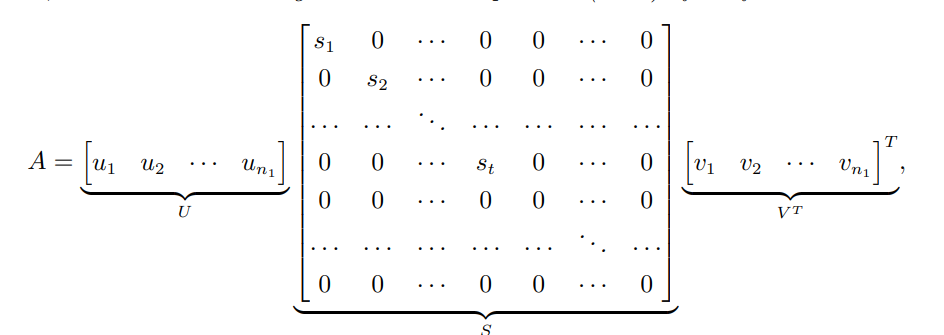
\includegraphics[width=10cm]{/home/buzgalbraith/work/school/spring_2023/probaility-theroy-2-2023/notes/week_10/video_!/images/v10_1.png}
\\ where  the singular values $s_1\geq s_2 \geq \cdots \geq s_t$ are positive real numbers, the left singular vectors
$u_1,u_2\cdots u_r\in \mathbb{R}^{n_1}$ are orthonormal and the right singular vectors $v_1,v_2\cdots v_r\in \mathbb{R}^{n_2}$

\item proof
\begin{enumerate}
    \item first it is clear that for an arbitrary matrix $A\in \mathbb{R}^{n_1\times n_2}$ we can write a symmetric matrix as $M:=AA^{T}\in \mathbb{R}^{n_1\times n_1}$
    \item and further by the spectral theorem we know that any symmetric matrix can be eiegen decomposed and thus has $n_1$ orthonormal vectors $u_1,\cdots , u_{n_1}$
    \item further note that the corresponding eigenvalues $\lambda_{n_1}$ are non-negative since $0> ||A^{t}u_{j}||_{2}^{2}=u_{j}^{t}AA^{t}u_{j}=u_{j}^{t}Mu_{j}=\lambda_{j}u_{j}^{t}u_{j}=\lambda_{j}$ that is positive definite
    \item and further the number of non-zero eigenvalues is equal to teh rank of A, and further because A and $AA^{T}$ have he same rank  
    \item the  number of non-zero eigen values of $m$ is equal to the rank of a, and since A and $A^{t}$ have the same number of eigenvalues call if $t$ we have $s_{t}:=\sqrt{\lambda_{t}}$ and $$v_{t}:=\frac{1}{s_{t}}A^tu_{1}$$
    \item further these vectors have unit norm $$||v||_{2}^{2}=\frac{1}{s_{1}^2}u_{1}^{t}AA^{T}u_{1}=\frac{\lambda _t}{\lambda_t}u_{1}^{T}u_{1}=1$$
    \item further all the singular vectors are orthogonal
    \item so we can define the fallowing matrices $$U:[u_1\cdots u_{n_1}]$$ $$V:[v_1\cdots v_{n_1}]$$ such that $$U^TA=SV^T$$
    notice here that U is orthogonal  matrix as it is square an has orthomonal columns thus $UU^{T}$ meaning that $$A=USV^T$$
\end{enumerate}
\item the rank of a matrix is equal to the number of non singular eigenvalues
\item we can write any matrix as a linear combination of rank 1 matrices as $$D=\Sigma_{l=1}^{n_1}S_{i}K_{l}=\Sigma_{l=1}^{n_1}s_{l}u_{l}v_{l}^{T}$$
\item the rank of matrix $K_{l}$ is one because it is the outter product of the left singular vector $u_{l}$ and the right singular vector $v_{l}$ so its ellements are scalled coppies of the two. 
\item the rank 1 matrices are orthogonal and have unit norm 
\item \textbf{the Frobenius inner product } of two matrices $A\in \mathbb{R}^{n_1\times n_2}$ and $B\in \matbn{R}^{n_1\times n_2}$ is $$<A,B>:=\Sigma_{i=1}^{n_1}\Sigma_{j=1}^{n_2}A[i,j]B[i,j]=Trace(A^TB)$$
where the trace is the sum of its diagonal enteries. the coresponding norm is 
$$||A||_{F}=\sqrt{{A,A}}=\sqrt{trace(A^TA}$$
\item if we vectorize the matricies that is concatange the coloumns into vectors the f norm is equivlent to the $l_{2}$ norm 
\item the rank 1 matricies $K_1\cdots K_n_{1}$ form an orthonmal set with respect to teh forbinus inner product and norm 
\item in SVD eaech rank 1 matrix $K_{l}$ with unit f norm is weighted by the coresponding singular value $s_1$
\item for any matrix $A\in \mathbb{R}^{n_1\times n_2}$ with singular values $s_1\cdots s_min{n_1,n_2}$ $$||A||_{F}=\sqrt{\Sigma_{i=1}^{min(n_1,n_2} s_{i}^2}$$
\item to see this assume that $n_1\leq n_2$ (if this fails we can do the same argument on the transpose of a)
\item we denote the SVD of a as $A=\Sigma_{i=1}^{n_1}s_{i}K_{i}=\Sigma_{i=1}^{n_1}s_{i}u_{i}V_{i}^{t}$
\item we know that the rank one matrcies $K_{l}$ are orthogonol so by the pythagron therome we have $$||A||_{f}^{2}=||\Sigma_{l=1}^{n_1}s_lK_L||_{f}^{2}=\Sigma_{l=1}^{n_1}s_l||K_L||_{f}^{2}=\Sigma_{l=1}^{n_1}s_l$$
\subsection{truncating the singular value decomposition}
\item as we know that the total f norm of the svd is the sum of the squared signual values, the magintures of the singlar values allow us to qunatify the contribution of each component to the dataaset
\item this sugests a simple low rank aproximation of our data set would be to simply take the r largest singular values of the matrix 
\item so consider the truncated svd $$L_{SVD}:=\Sigma_{i=1}^{r}s_{l}K_{l}=\Sigma_{l=1}^{r}s_lu_lv_l^t$$
\item we can compute the aproximation erorr of this low rank model as $$||D-L_{svd}||_{f}^{2}=||\Sigma_{l=r+1}^{n_1}||_{f}^{2}=\Sigma_{l=r+1}^{n_1}s_{l}^2$$ that is the error is the sum of the squared singular values we are not taking 
\subsection{SVD and PCA}
\item we can show that PCA and SVD yield the same low rank aproximation 
\item let $D\in \mathbb{R}^{n_1\times n_2}$ be an arbitary matrix what has been centerd by subtracting it's mean entery. let r be a postive integer smaller than $n_1, n_2$ we denote the coloumn wise rank r pca aproximation of $D$ by


































\item
consider arbitrary matrix $D\in \mathbb{R}^{n\times d}$. (which has been centred by subtracting it's mean entry)
\item let $r\in \mathbb{Z}:r<min(n,d)$
\item the column wise pca rank r of D is given by $$L_{pca-col}:=\Sigma_{l=1}^{r}u_{l}w_{l}$$ where $w_{l}[j]=u_{l}^{t}D[:,j]: j\in [1,d]$ and $u_l\in [1,r]$ is the eigin vector of the sample covariance matrix $\Sigma_{cols}:=\frac{1}{n^2}DD^T$
\item the rank wise pca rank r of D is given by $$L_{pca-row}:=\Sigma_{l=1}^{r}u_{l}w_{l}$$ where $w_{l}[j]=u_{l}^{t}D[:,j]: j\in [1,d]$ and $u_l\in [1,r]$ is the eigin vector of the sample covariance matrix $\Sigma_{cols}:=\frac{1}{n^2}DD^T$
\item let $D=USV^T$ be the dvd of F. the coloum wise smaple covaraince matirx can be expressed as 
$$\Sigma_{cols}:=\frac{1}{d}DD^t=\frac{1}{d}USV^t(USV^t)^t=\frac{1}{d}USV^T VS^TU^T=\frac{1}{d}USS^TU^T$$ given that we know S is a diagonal matrix we can write 
$$\frac{1}{d}USS^TU^T=U\frac{1}{d}S^2U^T$$ which is equal to diagonal eigen matrix of the squared singular values of D. further this is how we defined our left sinfular values of D t thus we can see that the largest r egienvectors of $\Sigma_{cols}$ are equal to the first r left singular vectors of D 
\item so furhter we can write $w_{l}[j]=s_{l}v_{l}(j)$
\item then by this we can write $l_{plca-cols}[i,j]=\Sigma_{l=1}^{r}u_{l}[i]w_{l}[j]=\Sigma_{l=1}^{r}s_{l}u_{l}[i]v_{l}[j]=L_{svd}[i,j]$
\item and we can show this olds holds row wise 
\subsection{otpimal low rank matrix estimation}
\item here we are going to prove that the rank r approximation obtained using the truncated svd is optimal with respect to the f norm 
\item suppose twe have to matricies $A,B\in \mathbb{R}^{n\times d}$ such that there col spaces are orthogonal that is $$<a,b>=trace(A^TB)=\Sigma_{i=1}^{d}<A[:<i], B[:,i]>=0$$ that is there column are pairwise independent 
\item then by the pythogean therome we have $$||A+B||_{f}^{2}=||A||_{f}^{2}+||B||_{f}^{2}$$ given they have orthogonol col spaces
\item consider the  $D$ $0<r\leq min(n,d)$
\item let U be a matrix with r orthognal cols that span teh coloumn sapc of d such that $UU^TD=D$ the low random aproximation $UU^TD$ obtrained by pojecting teh colmns of d onto teh col space of l can nly imporve the apromixation error 
$$||D-L||_{f}^{2}$$
\item i dont have time to finish typing tehse notes up right now sorry. 

\end{itemize}
\end{document}
